\documentclass[aps, 10pt, preprintnumbers, prd, amsmath, amssymb,twocolumn, notitlepage, nofootinbib]{revtex4} %, ,10pt

%\documentclass[aps, 10pt, preprintnumbers,prd, amsmath,amssymb,notitlepage]{revtex4} %, ,10pt
\usepackage{graphicx}% Include figure files latexsym,array,enumerate,letter,numbers,twocolumn
%\usepackage{dcolumn}% Align table columns on decimal point
\usepackage{bm}% bold math
%\usepackage{amssymb}
\usepackage{subfigure}
\usepackage{epsfig}
%\usepackage{slashed}
\usepackage{color}
%\usepackage{cite}
\usepackage{mathtools}
\usepackage{cases}
\usepackage{booktabs}
\usepackage{amsmath}
%\usepackage{subcaption}

\usepackage[
colorlinks=true,
filecolor=black,
anchorcolor=blue,
linkcolor=blue,
citecolor=cyan, %red,
urlcolor=cyan,
linktocpage=true,
plainpages=false,
breaklinks=true,
pdfstartview=FitH
]{hyperref}

\def\cd{\color[rgb]{0.00,0.50,0.25}} %delete
\def\cm{\color[rgb]{0.00,0.60,0.00}} %modify
\def\cn{\color[rgb]{0.80,0.00,0.40}} %
 
\def\m{{\cm\mu_0}}
\def\e{{\cm\epsilon_0}}

% define some useful aliases
\newcommand{\kbh}{k_{\r{bh}}}
\newcommand{\sbh}{\sigma_{\r{bh}}}
\newcommand{\mbh}{m}
\newcommand{\neff}{N_{\rm{eff}}}
\newcommand{\dneff}{\Delta N_{\rm{eff}}}
\newcommand{\ms}{m_{\odot}}
\newcommand{\fbh}{f_{\r{bh}}}
\newcommand{\GW}{\Omega_\r{GW}}
\newcommand{\rd}{\r{d}}
\DeclareRobustCommand{\Eq}[1]{Eq.~(\ref{#1})}
\DeclareRobustCommand{\Fig}[1]{Fig.~\ref{#1}}

\newcommand{\ps}{P_{\mathcal{R}}}
\def\di{\mathrm{d}}

\def\eps{\epsilon}
%\def\d{\partial}
\def\l{\left(}
\def\r{\right)}
\def\la{\langle }
\def\ra{\rangle }



\newcommand{\ck}[1]{\textcolor{blue}{#1}}
\newcommand{\ckk}[1]{\textcolor{red}{#1}}
\newcommand{\vev}[1]{\left<{#1}\right>}
\newcommand{\bra}[1]{\left|{#1}\right>}
\newcommand{\ket}[1]{\left<{#1}\right|}


\newcommand{\E}{\mathbf{E}}
\newcommand{\B}{\mathbf{B}}
\newcommand{\J}{\mathbf{J}}
\newcommand{\Mpl}{M_{\rm Pl}}
\newcommand{\n}{\mathbf{n}}

\newcommand{\ab}{\alpha \beta}
\newcommand{\mn}{\mu \nu}
\newcommand{\rs}{\rho \sigma}
\newcommand{\hmn}{h_{\mu \nu}}
\newcommand{\TT}{\text{TT}}
\newcommand{\jeff}{j_\text{eff}}
\newcommand{\hnorm}{h_0}
\newcommand{\order}[1]{\mathcal{O}{(#1)}}
\newcommand{\nl}{\nonumber \\}
\newcommand{\w}{\omega}
\newcommand{\wg}{\omega_g}
\newcommand{\lamg}{\lambda_g}
\newcommand{\tTT}{t_{_\text{TT}}}
\newcommand{\xTT}{x_{_\text{TT}}}
\newcommand{\yTT}{y_{_\text{TT}}}
\newcommand{\zTT}{z_{_\text{TT}}}
\newcommand{\UTT}{U_{_\text{TT}}}
\newcommand{\jTT}{j_{_\text{TT}}}
\newcommand{\FTT}{F_{_\text{TT}}}
\newcommand{\fTT}{f_{_\text{TT}}}
\newcommand{\grad}{\nabla}

\newcommand{\jveff}{\boldsymbol{j}_\text{eff}}
\newcommand{\jvhat}{\hat{\jv \, }}
\newcommand{\jplus}{\jvhat_{\hspace{-0.1 cm} +}}
\newcommand{\jcross}{\jvhat_{\hspace{-0.1 cm} \times}}
\newcommand{\jpc}{\jvhat_{\hspace{-0.1 cm} +, \times}}

\newcommand{\emu}{\hat{\mathbf{e}}_\mu}
\newcommand{\enu}{\hat{\mathbf{e}}_\nu}
\newcommand{\erho}{\hat{\mathbf{e}}_\rho}
\newcommand{\ephi}{\hat{\mathbf{e}}_\phi}
\newcommand{\ez}{\hat{\mathbf{e}}_z}
\newcommand{\ex}{\hat{\mathbf{e}}_x}
\newcommand{\ey}{\hat{\mathbf{e}}_y}
\newcommand{\rv}{\mathbf{r}}
\newcommand{\vv}{\mathbf{b}}
\newcommand{\jv}{\mathbf{j}}
\newcommand{\rvp}{\mathbf{r'}}
\newcommand{\Rv}{\mathbf{R}}
\newcommand{\al}{S_\text{\scriptsize loop}}
\newcommand{\at}{S_\text{\scriptsize toroid}}
\newcommand{\rl}{\rho_\text{\scriptsize loop}}
\newcommand{\rt}{\rho_\text{\scriptsize max}}
\newcommand{\rmi}{\rho_\text{\scriptsize min}}
\newcommand{\bmax}{B_{\text{max}}}

\newcommand{\be}{\begin{equation}}
\newcommand{\ee}{\end{equation}}
\newcommand{\bea}{\begin{equation}\begin{aligned}}
\newcommand{\eea}{\end{aligned}\end{equation}}
\newcommand{\ga}{g_{a\gamma\gamma}}
\newcommand{\bE}{\mathbf{E}}
\newcommand{\bB}{\mathbf{B}}
\newcommand{\bP}{\mathbf{P}}
\newcommand{\bM}{\mathbf{M}}
\newcommand{\bk}{\mathbf{k}}
\newcommand{\bU}{\mathbf{U}}
\newcommand{\bV}{\mathbf{V}}
\newcommand{\rhoDM}{\rho_{\scriptscriptstyle \textrm{DM}}}
\newcommand{\PBH}{{\scriptscriptstyle \textrm{PBH}}}
\newcommand{\hTT}{h^{\scriptscriptstyle \textrm{TT}}}
\DeclareRobustCommand{\r}[1]{{\rm #1}}

\newcommand{\xv}{{\bf x}}
\newcommand{\Vcav}{V_\text{cav}}


%math symbols
\newcommand{\curl}{\nabla\times}

%math symbols
%\newcommand{\curl}{\nabla\times}
\begin{document}

\title{Implications for High Frequency Gravitational Wave from the PTA Data}
\author{Junsong Cang$^{1}$}
\email{cangjunsong@outlook.com}
\author{Yu Gao$^{2}$}
\email{gaoyu@ihep.ac.cn}
\author{Yi-ming Liu$^{3}$}
\email{7520220161@bit.edu.cn}
\author{Sichun Sun$^{3}$}
\email{sichunssun@bit.edu.cn}


\affiliation{$^1$ School of Physics, Henan Normal University, Xinxiang, China}
\affiliation{$^{2}$Key Laboratory of Particle Astrophysics, Institute of High Energy Physics,
Chinese Academy of Sciences, Beijing 100049, China}
\affiliation{School of Physics, Beijing Institute of Technology, Beijing, 100081, China}


\begin{abstract}
Recently several pulsar timing array (PTA) experiments such as NANOGrav and PPTA reported detection of a gravitational wave (GW) background at nano-Hz frequency band.
Enhanced curvature perturbation $\ps$ can produce scalar induced gravitational wave (SIGW) that serves as a good source candidate for the observed GW signal.
Here we show that if the PTA signal were indeed of SIGW origin,
$\ps$ amplitude required will produce primordial black holes (PBHs) in $[2 \times 10^{-5}, 2 \times 10^{-2}]\ m_\odot$ mass range.
Mergers of these PBHs will produce strong gravitational wave (GW) background in $[10^{-3}, 10^8]$ Hz frequencies that falls into the sensitivity reach of various high frequency GW observatories such as 
the Einstein Telescope (ET),
DECIGO and BBO,
which can help further scrutinize the SIGW interpretation of PTA signal.

\end{abstract}

\maketitle

\ck{\it Introduction}
Enthusiasm in primordial black holes (PBHs)~\cite{Zeldovich:1967lct,Carr:1974nx} has grown immensely after the LIGO discovery of gravitational wave signals~\cite{LIGOScientific:2018mvr} in agreement with merger events of black holes above stellar masses~\cite{Bird:2016dcv}.
With sufficiently large primordial curvature perturbation $\mathcal{R}$,
such black holes can be produced in the early Universe from gravitational collapse of overdense regions.
PBHs are under extensive searches for their astrophysical signals,
see Ref.~\cite{Carr:2021bzv} for a recent review.
%If produced in abundance, 
%PBHs can leave footprints that can be tested through astrophysical searches.
The early process of over-density collapse is also predicted to release scalar-induced gravitational waves (SIGW)~\cite{Domenech:2021ztg,Cang:2022jyc},
which offers a glimpse at valuable information of early fluctuations at late-time gravitational wave detectors.

{\color{blue}
The primordial black hole can be supermassive, to generate gravitational waves from the mergers directly. 
In the case of the scalar-induced gravitational waves(SIGW), 
the associated PBH produced in this case is a couple of orders below solar mass, 
and the mergers of such light PBH produced a gravitational wave signal around Mhz. 
Since the endeavor of the whole gravitational wave frequency spectrum searches has begun, 
with various proposals already in Mhz-Ghz band\cite{Domcke:2022rgu}, 
it is intriguing to link the ultra-low NanoHz gravitational waves to the ultra-high frequency gravitational searches. 
We may call it a multi-messager task in the frequency spectrum space.
}

In recent month, 
several Pulsar Timing Array (PTA) observatories including NANOgrav~\cite{NANOGrav:2023gor}, 
Chinese PTA (CPTA)~\cite{Xu:2023wog},
Parkes PTA (PPTA)~\cite{Reardon:2023gzh}
and European PTA~\cite{EPTA:2023gyr,EPTA:2023fyk}
reported strong evidence for gravitational wave (GW) background at nano-Hertz waveband,
which verifies previous claims from~\cite{NANOGrav:2020bcs, Chen:2021rqp, Goncharov:2021oub, Antoniadis:2022pcn}.
These observations incited several studies on potential sources of observed GW background~\cite{Franciolini:2023pbf},
such as supermassive black holes~\cite{NANOGrav:2023hvm,Middleton:2020asl}, 
phase transition~\cite{Bian:2020urb,NANOGrav:2021flc,Xue:2021gyq,Wang:2022wwj} and 
axion topological defects~\cite{Wang:2022rjz,Ferreira:2022zzo,Inomata:2023drn}.


%In recent years, 
%several Pulsar Timing Array (PTA) observatories including NANOgrav~\cite{NANOGrav:2020bcs}, 
%Parkes PTA (PPTA)~\cite{Goncharov:2021oub}, 
%European PTA~\cite{Chen:2021rqp} and a joint study ~\cite{Antoniadis:2022pcn} reported strong indication of a common-spectrum process in the 1-10 nano-Hertz waveband. 
%These claims are then strengthened in recent months,
%as various PTA datasets from NANOGrav~\cite{NANOGrav:2023gor},
%Chinese PTA (CPTA)~\cite{Xu:2023wog},
%International PTA (IPTA)~\cite{Antoniadis:2022pcn} and PPTA~\cite{Reardon:2023gzh}
%reported evidence for gravitational wave (GW) background at high confidence levels.
%These observations incited several studies on a potential signal from supermassive black holes~\cite{NANOGrav:2023hvm,Middleton:2020asl}, 
%or from more cosmological origins, 
%such as phase transition~\cite{Bian:2020urb,NANOGrav:2021flc,Xue:2021gyq,Wang:2022wwj} and axion topological defects~\cite{Wang:2022rjz,Ferreira:2022zzo,Inomata:2023drn}.
%%Continued PTA observations are expected to verify the robustness of the earlier claim. 

In case of SIGW from overdensity collapse, 
a GW signal at PTA's nHz frequency generally requires a curvature power spectrum $\ps$ with large amplitude at the scale of $k\sim 10^{8}$ Mpc$^{-1}$~\cite{Franciolini:2023pbf,NANOGrav:2023hvm}.
At large scales ($k \lesssim 10 \r{Mpc^{-1}}$),
$\ps$ has been well constrained by observations from cosmic mircrowave background (CMB) and large scale structures~\cite{Hunt:2015iua,Planck:2018vyg},
however at smaller scales $\ps$ is comparably poorly constrained~\cite{Cang:2022jyc} and can potentially has amplitude large enough to explain PTA signal.

In this letter,
we show that $\ps$ amplitude required for generating SIGW compatible with PTA data will also lead to formation of PBHs with mass in $[2\times 10^{-5}, 2 \times 10^{-2}] m_\odot$ range.
The mergers of these PBHs can produce GW background peaked at around MHz frequencies,
which can be easily detected by various high frequency GW observatories such as Einstein Telescope (ET)~\cite{Punturo:2010zz},
Deci-Hertz Interferometer Gravitational Wave Observatory (DECIGO)~\cite{Kawamura:2020pcg} and Big Bang Observer (BBO)~\cite{Yagi:2011wg}.
This work is structured as follows,
we begin by a review of our model for SIGW and merging PBH.
After discussing our inference settings we present our results and conclusions.

%In this paper, we adopt a log-normal power spectrum in the XXX model, and we show the latest NANOgrav result is in cosistency with ... We also discuss the abundance of the associately produced PBHs in the same process.



%in the  that behave like an extra radiation component,
%thus contributing to the relativistic degrees of freedom ($\neff$).
%We show that the cosmological constraints on $\neff$ can be used to pose stringent limits on PBHs created from this particular scenario as well as the relevant small-scale curvature perturbation ($\ps(k)$).

\ck{\it GW from curvature perturbation and PBH mergers. }
As a good approximation for a large class of curvature perturbation models,
we consider a log-normal parameterization for curvature power spectrum $\ps$
~\cite{Inomata:2018epa, NANOGrav:2023hvm, Franciolini:2023pbf, Pi:2020otn, Chen:2021nio},
\be
\ps
=
\frac{A}{\sqrt{2 \pi \Delta^2}}
\exp
\left[
-\frac{(\ln k/k_*)^2}{2\Delta^2}
\right]
\label{dsf9887hdsf}
\ee
where $A,\ k_*$ and $\Delta$ are model parameters,
which describe the amplitude,
peak location and the width of $\ps$ respectively.
Upon horizon crossing,
$\ps$ will modify the radiation quadruple moment and generate SIGW at second order.
If sufficiently large,
$\ps$ will also generate overdense regions that can gravitationally collapse and form PBHs~\cite{Cang:2022jyc}.
Here we find that the PBHs generated by $\ps$ spectrum in \Eq{dsf9887hdsf} has a mass distribution that can be well fit by a log-normal profile~\cite{Cang:2022jyc},
\be
\psi
=
\fbh
\frac{1}{\sqrt{2 \pi} \sbh}
\exp
\left[
-
\frac{\r{ln}^2(\mbh/m_{\r{c}})}
{2 \sbh^2}
\right]
,
\label{dshiuy65}
\ee
where $\psi \equiv {\r{d}\fbh}/{{\rm d} \ln \mbh}$,
$\fbh \equiv \rho_\r{bh}/\rho_\r{dm}$ is the fraction of DM made of PBHs,
$\rho_\r{bh}$ and $\rho_\r{dm}$ denotes mass densities of PBH and DM respectively,
$m$ denotes PBH mass,
$m_\r{c}$ and $\sigma_\r{bh}$ are peak and width of the distribution respectively.
For convenience,
in what follows we will parameterise our PBH distribution using \Eq{dshiuy65}.

%Note that it's often convenient to describe PBH distribution via number density rather than mass density in \Eq{dshiuy65},
%\be
%\begin{aligned}
%\Psi
%&\equiv
%\frac{1}{n_\r{bh}}
%\frac{\rd n_\r{bh}}{\rd \ln m}
%\\
%&=
%\frac{\left<\mbh\right>}{\mbh}
%\frac{1}{\sbh \sqrt{2 \pi}}
%\exp
%\left[
%-
%\frac{\r{ln}(\mbh/m_{\r{c}})^2}
%{2 \sbh^2}
%\right]
%\end{aligned}
%\ee
%
%\be
%\begin{aligned}
%\left<
%\mbh
%\right>
%&\equiv
%\frac{\rho_{\r{bh}}}
%{n_{\r{bh}}}
%\\
%&=
%\left[
%\frac{1}{\sqrt{2 \pi} \sbh}
%\int
%\frac{\rd \ln \mbh}
%{\mbh}
%\exp
%\left[
%-
%\frac{\r{ln}(\mbh/m_{\r{c}})^2}
%{2 \sbh^2}
%\right]
%\right]^{-1}
%\end{aligned}
%\ee

%\section{GW from PBH merger}
In addition to SIGW,
merger events of PBH binaries created by $\ps$ can also emit GW at higher frequencies.
The comoving merger rate $R$ of a pair of PBHs with mass $m_1$ and $m_2$ is given by~\cite{Raidal:2018bbj},
%\footnote{
%Note that the mass function $\psi$ is defined as $\rd \ln \fbh/\rd \ln \mbh$ in~\cite{Raidal:2018bbj}
%},
\be
\begin{aligned}
\frac{\rd R}{\rd m_1 \rd m_2}
&\simeq
\frac{1.6 \times 10^6}
{\r{Gpc^3 yr}}
\fbh^{-\frac{21}{37}}
\eta^{-\frac{34}{37}}
\left(
\frac{M}{m_\odot}
\right)^{-\frac{32}{37}}
\\
&
\times
\left(
\frac{t}{t_0}
\right)^{-\frac{34}{37}}
S
\psi(m_1)
\psi(m_2)
\end{aligned}
\label{dfiiuiu7thxdcyeg63}
\ee
where 
$M = m_1 + m_2$,
$\eta = m_1 m_2 / M^2$,
$t$ is the time of merger,
$t_0 = 13.8 \r{Gyr}$ is the current age of the Universe.
$S$ is a suppression factor which takes the form~\cite{Raidal:2018bbj, Hutsi:2020sol},
%\be
%S = S_1 \times S_2
%\ee
\be
\begin{aligned}
S
&=
\frac{\r{e}^{-\bar{N}(y)}}
{\Gamma(21/37)}
\int \rd v
v^{-\frac{16}{37}}
\exp
\left[
-
\phi
-
\frac{3 \sigma^2_\r{M} v^2}
{10 \fbh^2}
\right]
\end{aligned}
\label{fdvdsx2rsdcvio}
\ee
\be
\phi
=
\frac{
\bar{N}(y)
\left<
m\right>
}
{\fbh}
\int
\frac{\rd \mbh}{\mbh}
\psi(m)
F
\left(
\frac{M}
{
\left<
m
\right>
}
\frac{v}
{\bar{N}(y)}
\right)
\ee
where 
$\sigma_\r{M} \simeq 0.004$,
$\bar{N}(y)$ is the expected number of PBHs within a comoving radius of $y$ around the binary~\cite{Hall:2020daa},
and we take 
$\bar{N}(y) \simeq
{M \fbh}
/
[
\left<m\right>
(\fbh + \sigma_\r{M})]
$
following~\cite{Raidal:2018bbj,Hutsi:2020sol,Hall:2020daa},
which has been shown to agree well with numerical simulation for $\fbh \le 0.1$~\cite{Raidal:2018bbj,Hall:2020daa}.
$\left<m\right>$ is the mean of PBH mass over number density distribution~\cite{Hutsi:2020sol},
which equals $m_\r{c} \r{e}^{-\sbh^2/2}$ for our log-normal mass distribution in \Eq{dshiuy65}.
$
F(z)
=_1F_2
(-1/2,3/4,5/4;-9z^2/16)
-1
$,
$_1F_2$ is the generalized hypergeometric function.

%\be
%\bar{N}(y)
%\simeq
%\frac{M}
%{\left<m\right>}
%\frac{\fbh}
%{\fbh + \sigma_\r{M}}
%\ee
%
%\be
%\begin{aligned}
%\left<
%m
%\right>
%&\equiv
%\fbh
%\left[
%\int \rd \ln\mbh
%\ 
%\frac{\psi}{\mbh}
%\right]^{-1}
%\\
%&=
%m_\r{c}
%\r{e}^{-\sbh^2/2}
%\end{aligned}
%\ee

The energy density for merging PBHs is calculated as~\cite{Depta:2023qst},
\be
%\frac{{\rm d}\Omega_{\rm MGW}}{{\rm d}\ln f}
\GW
%\Omega_\r{GW}
=
\frac{f}{\rho_\r{cr}}
\int \frac{\rd z \rd R}
{(1+z)H}
\frac{\rd E_\r{GW}(f_\r{r})}
{\rd f_\r{r}}
\ee
here $\Omega_\r{GW} \equiv \rho^{-1}_\r{cr} \rd \rho_\r{GW} / \rd \ln f$ is fractional GW density per log frequency interval,
$\rho_\r{GW}$ and $\rho_\r{cr}$ are GW density and current critical density respectively,
$f_\r{r} = (1+z)f$ is the source frequency,
$\rd E_{\r{GW}}(f_\r{r})/\rd f_\r{r}$ is the source energy spectrum for each individual PBH merger event,
for which we adopt~\cite{Zhu:2011bd},
$H = H_0[\Omega_\Lambda + \Omega_\r{m}(1+z)^3 + \Omega_\r{r}(1+z)^4]^{1/2}$ denotes Hubble parameter,
and we use the Planck 2018~\cite{Planck:2018vyg} of $H_0 = 67.66\ \r{km s^{-1}Mpc^{-1}}$,
$\Omega_\Lambda = 0.6903$ and 
$\Omega_\r{m} = 0.3096$.
We assume massless neutrino such that the radiation density fraction $\Omega_\r{r} =9.1 \times 10^{-5}$.

%\be
%\begin{aligned}
%\frac{\rd E_\r{GW}(f_\r{r})}
%{\rd f_\r{r}}
%&=
%\frac{
%(\pi G)^{2/3}
%M^{5/3}
%\eta
%}
%{3}
%\\
%&
%\times
%\left\{
%\begin{array}{l}
%f^{-1/3}_\r{r}
%,
%\ \ \ \ \ \ \ \ \ \ \ \ \ \ \ \ \ \ \ \ \ \ \ \ \ \ \ \  f_\r{r} < f_1\\
%\\
%\frac{f^{2/3}_\r{r}}
%{f_1}
%,
%\ \ \ \ \ \ \ \ \ \ \ \ \ \ \ \ \ \ \ \ \  \ \ \ \ \ \  f_1 \le f_\r{r} < f_2\\
%\\
%\frac{f^2_\r{r}}
%{f_1 f_2^{4/3}}
%\frac{f_4^4}
%{\left(
%4(f_\r{r}
%-f_2
%)^2
%+
%f_4^2
%\right)^2
%}
%,  
%\ \ \ \ \  f_2 \le f_\r{r} < f_3\\
%\end{array}
%\right.
%\end{aligned}
%\label{eqdsfgr89inja}
%\ee
%here $f_i = (a_i \eta^2 + b_i \eta + c_i)$,
%the polynomial coefficients $a_i,\ b_i, c_i$ are taken from~\cite{Ajith:2007kx,Depta:2023qst} and we list them all here in 
%Tab.\ref{t456h3wedfghsa}.
%\begin{table}[htp]
%\begin{tabular}{c|ccc}
%\hline
%  & a & b & c\\
%\hline
%$f_1$ & $2.9740 \times 10^{-1}$ & $\ \ \ 4.4810 \times 10^{-2}$ & $\ \ \ 9.5560 \times 10^{-2}$\\
%$f_2$ & $5.9411 \times 10^{-1}$ & $\ \ \ 8.9794 \times 10^{-2}$ & $\ \ \ 1.9111 \times 10^{-1}$\\
%$f_3$ & $8.4845 \times 10^{-1}$ & $\ \ \ 1.2848 \times 10^{-1}$ & $\ \ \ 2.7299 \times 10^{-1}$\\
%$f_4$ & $5.0801 \times 10^{-1}$ & $\ \ \ 7.7515 \times 10^{-2}$ & $\ \ \ 2.2369 \times 10^{-2}$\\
%\hline
%\end{tabular}
%\caption{
%Polynomial coefficients for characteristic frequencies $f_1,\ f_2,\ f_3$ and $f_4$ in 
%\Eq{eqdsfgr89inja}.
%}
%\label{t456h3wedfghsa}
%\end{table}

\ck{\it Inference Settings}
To find the credible region for PBHs and the corresponding merger GW signal,
we analyzed the PTA datasets using our SIGW model.
Our log-likelihood takes the form,
\be
\ln \mathcal{L}
=
-\frac{1}{2}
\sum_{i}
\frac{(x_i - u_i)^2}{\sigma_i^2}
\label{dshf3765rghfdv}
\ee
here the index $i$ denotes frequency,
$x$ is $\Omega_\r{GW}$ for our SIGW model,
$u$ is the measured median for $\Omega_\r{GW}$,
$\sigma$ is the error bar for $\Omega_\r{GW}$,
which equals $\sigma_u$ for $x>u$ and $\sigma_l$ otherwise,
where $\sigma_u$ and $\sigma_l$ are upper and lower error bars respectively.
We used PTA GW datasets from NanoGrav~\cite{NANOGrav:2023gor}, 
IPTA~\cite{Antoniadis:2022pcn} and PPTA~\cite{Reardon:2023gzh} in our inference.
For convenience,
we follow~\cite{Franciolini:2023pbf} and estimate the signal median and error bars for each experiment directly using 
the $\Omega_\r{GW}$ posterior summarised in~\cite{Franciolini:2023wjm,Li:2023yaj},
and we have checked that our results (when using NG15 data only) agrees very well with that shown in~\cite{Franciolini:2023pbf} and~\cite{NANOGrav:2023hvm} .

As a form of dark radiation,
the extra energy budget from SIGW will also change the effective degree of relativistic degrees of freedom $\neff$.
In Planck 2018 results (hereafter PLK)~\cite{Planck:2018vyg},
a joint analysis of datasets from CMB, 
baryon acoustic oscillations (BAO) and Big Bang Nucleosynthesi (BBN) constrain $\neff$ to~\cite{Planck:2018vyg,Cang:2022jyc},
\be
\dneff
\equiv
\neff - 
3.046
\le
0.175
,\ 95\%\ \r{C.L.}
\label{dsfhi38r767fdg}
\ee
this translates into an upper bound on integrated GW density of $\int \rd \ln f\Omega_{\r{GW}} < 2.1 \times 10^{-6}$~\cite{Cang:2022jyc},
here $3.046$ is the value of $\neff$ predicted by the standard model of particle physics~\cite{deSalas:2016ztq,Planck:2018vyg,Cang:2022jyc}.
%and $\Omega_\r{GW}$ is related to $\dneff$ by~\cite{Cang:2022jyc},
%\be
%\dneff
%=8.3 \times 10^4 
%\int \rd \ln f\Omega_{\r{GW}},
%\label{dsvuytdui}
%\ee
To accomodate the PLK $\neff$ limits,
we added a prior of $\dneff < 0.175$ to our inference.
Since $\fbh$ in our mass range has been constrained to $\mathcal{O}(0.1)$~\cite{Carr:2020xqk},
we also use a prior of $\fbh \in [10^{-20}, 10^{-1}]$,
this ensures that PBH does not violate the existing abundance constraints while still has physically meaningful abundance for appreciable merger GW production.
For completeness,
we consider a total of 3 inference settings:
\begin{itemize}
\item {\bf GW}: Use PTA GW data alone.
\item {\bf GW + $\dneff$}: Use PTA GW data and PLK $\dneff$ limits in \Eq{dsfhi38r767fdg}.
\item {\bf GW + $\dneff$ + PBH}: Use PTA GW data and PLK $\dneff$ limits along with the prior of $\fbh \in [10^{-20}, 10^{-1}]$.
\end{itemize}
%
%\begin{table}[htp]
%\begin{tabular}{c|c|c}
%\hline
%Parameters & Prior range & Best-fit\\
%\hline
%$\log_{10}A$& [-1.8, 0] & -0.81\\
%$\log_{10}(k_*/\r{Mpc^{-1}})$& [6.8, 9] & 8.1\\
%$\Delta$& [0, 4] & 1.25\\
%\hline
%$\Delta N_\r{eff}$&  $\le 0.175$ & 0.0134\\
%$\log_{10}f_\r{bh}$& [-20, -1] & -1\\
%$\log_{10}[m_\r{c}/m_\odot]$ & -- & -3.59\\
%$\sbh$ & -- & 0.54\\
%\hline
%\end{tabular}
%\caption{
%Parameters varied in our inference and their allowed range.
%Note that $A$, $f_*$ and $\Delta$ are our free model parameters,
%whereas $\Delta N_\r{eff}$ and $\fbh$ are parameters derived from $A$, $f_*$ and $\Delta$.
%The best-fit values shown in the third column are the maximum-likelihoods points from our main GW+$\dneff$+PBH setting,
%the marginalized mean and errors for these parameters can be found in \Fig{e2ftssaasadwu}.
%}
%\label{tabd76543wedfghsa}
%\end{table}

\begin{table}[htp]
\begin{tabular}{c|c|c|c}
\hline
Parameters & Prior & 95\% Limits & 95\% Limits\\
 & range & GW & GW+$\dneff$ + PBH\\
\hline
$\log_{10}A$& [-1.8, 0] & [-1.3, -0.0] & [-1.51, -0.63]\\
$\log_{10}(k_*/\r{Mpc^{-1}})$ & [6.8, 9.0] & [7.4, 9.0] & [7.2, 8.6]\\
$\Delta$& [0.02, 4] & [0.02, 2.2] & [0.02, 2.22]\\
\hline
$\log_{10}f_\r{bh}$& [-20, -1] & [-13.6,  10.2] & [-16.9, -1]\\
$\log_{10}[m_\r{c}/m_\odot]$ & -- & [-5.7, -2.1] & [-4.7, -1.7]\\
$\sbh$ & -- & [0.15, 1.17] & [0.08, 0.84]\\
$\Delta N_\r{eff}$&  $\le 0.175$ & $[0, 0.36] $ & [0.006, 0.014]\\
\hline
\end{tabular}
\caption{
Parameters in our inference and their allowed range and marginalised 95\% C.L. limits.
$A$, $k_*$ and $\Delta$ are our free model parameters,
whereas $\fbh,\ m_\r{c},\ \sbh$ and $\Delta N_\r{eff}$ are parameters derived from $A$, $k_*$ and $\Delta$.
Note that GW data alone overproduces PBHs by about 10 orders of magnitude.
}
\label{tabd76543wedfghsa}
\end{table}

\begin{figure*}[htp]
\centering
\subfigbottomskip=-500pt
\subfigure{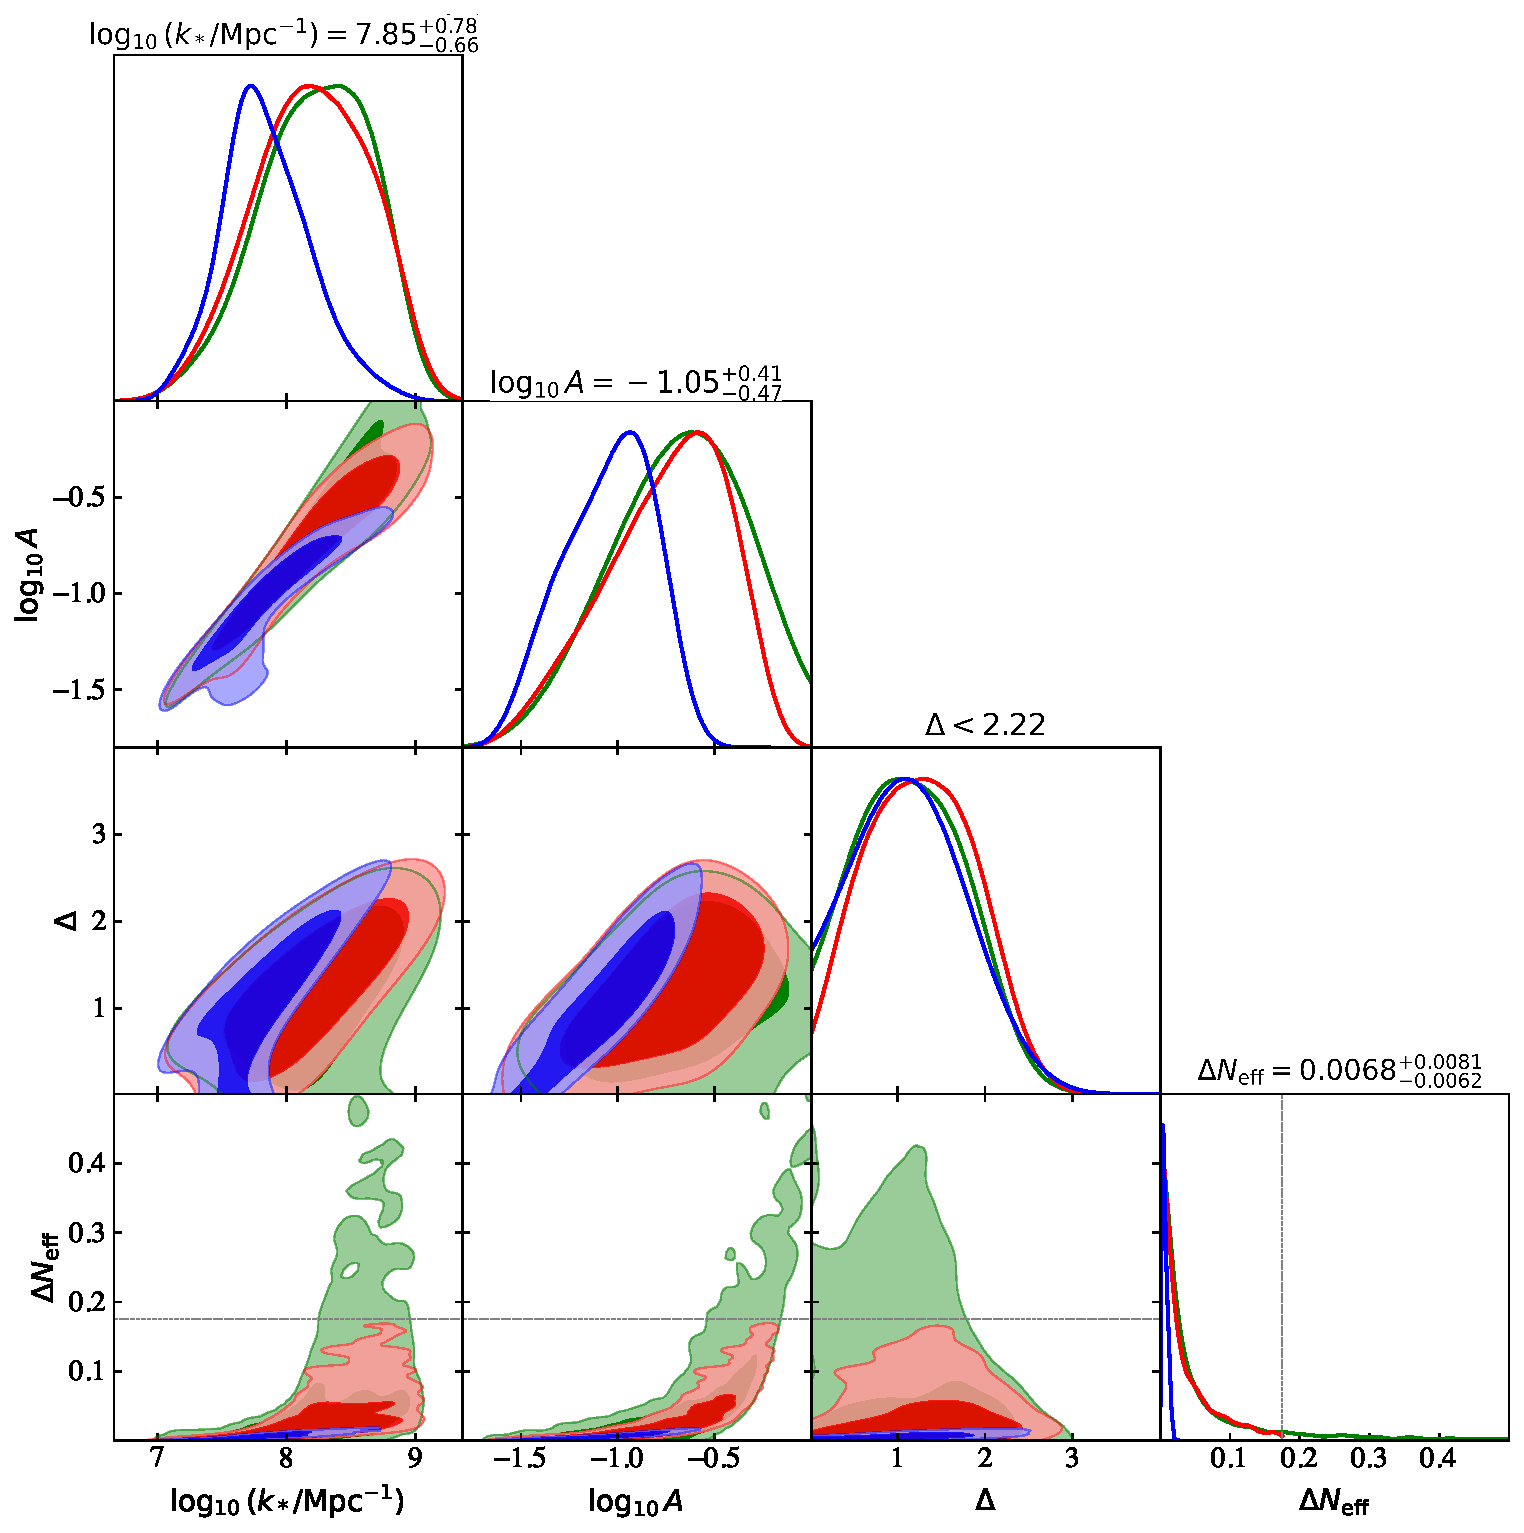
\includegraphics[width=8.5cm]{figs/param_posteriors.pdf}} \subfigure{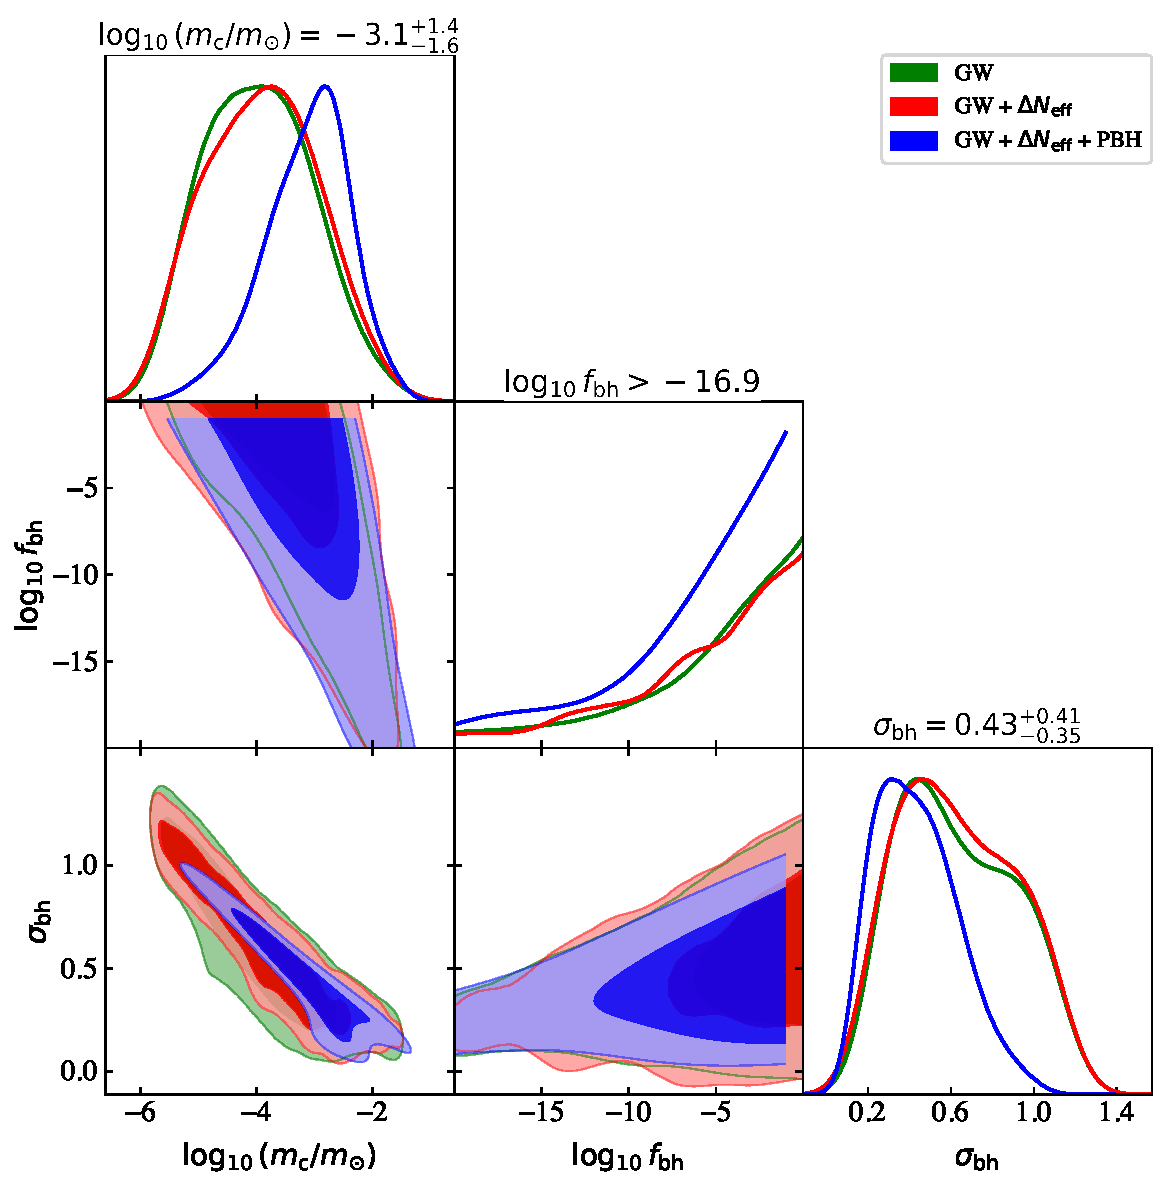
\includegraphics[width=8.5cm]{figs/PBH_posteriors_Full.pdf}}\\
\caption{
Marginalised posteriors for our $\ps$ parameters ($k_*,A,\Delta$) and the derived $\dneff$ and PBH parameters ($m_\r{c}, \fbh, \sbh$).
The green, red and blue contours correspond to GW, GW + $\dneff$, GW + $\dneff$ + PBH inference settings respectively.
Light and dark shaded regions correspond to 68\% and 95\% confidence levels respectively.
The dotted line in the $\dneff$ panels indicates the PLK upper limit of $\dneff < 0.175$,
numbers on the diagonal panels show the marginalised mean and 95\% confidence region from our main GW + $\dneff$ + PBH setting.
}
\label{e2ftssaasadwu}
\end{figure*}

\ck{\it Results}
We sampled the likelihoods in \Eq{dshf3765rghfdv} using the {\tt multinest} sampler~\cite{Feroz:2008xx},
and we compute constraints for our $\ps$ parameters and various derived observables (e.g. $\dneff$, PBH parameters and merger GW) by analyzing the  {\tt multinest}
chains using the {\tt GetDist} package~\cite{Lewis:2019xzd}.
Tab.\ref{tabd76543wedfghsa} summarises the prior ranges for our parameters along with their marginalised confidence region.
\Fig{e2ftssaasadwu} visualises the marginalised posterior from our inference,
the left panel shows the results for our $\ps$ model parameters and the derived $\dneff$ from different inference settings,
the right panel shows the results for PBH parameters $\fbh$, $m_\r{c}$ and $\sigma_\r{bh}$.

As can be seen from the left panel of \Fig{e2ftssaasadwu} and from Tab.\ref{tabd76543wedfghsa},
using GW data alone gives a marginalised $\dneff$ 95\% C.L upper bound of 0.36,
which is about $2\sigma$ away from the PLK upper limit,
%and the PBH peak mass $m_\r{c}$ and distribution width $\sbh$ are constrained to $[9.55 \times 10^{-06}, 9.8 \times 10^{-4}]\ m_\odot$
and adding the prior in \Eq{dsfhi38r767fdg} leads to a tighter constraints.
In both these inference settings,
the derived posterior for $\fbh$ can reach beyond the physically forbidden region of $\fbh\ge1$ by more than 10 orders of magnitude,
and after adding the physically motivated $\fbh < 0.1$ prior,
our constraints tightens significantly.
In GW fitting,
$m_\r{c}$ and $\sbh$ are constrained (at 95\% C.L.) to $[1.8 \times 10^{-6}, 7.5 \times 10^{-2}]\ m_\odot$ and $[0.15,\ 1.17]$ respectively,
and in the GW+$\dneff$+PBH fitting,
constraint tightens to $[2 \times 10^{-5}, 2 \times 10^{-2}]\ m_\odot$ for $m_\r{c}$ and $[0.08,\ 0.84]$ for $\sbh$.

In the green colored regions of \Fig{e2f8nb_asadwu},
we show the 95 \% C.L. posterior for the merger GW (left) and merger rate (right) derived from our main GW+$\dneff$+PBH inference,
and the black solid curves correspond to the maximum likelihood best-fit values of $\fbh = 0.1$, $m_\r{c} = 2.6 \times 10^{-4} m_\odot$ and $\sbh = 0.54$.
Our $\Omega_\r{GW}$ posterior peaks at around 10 MHz with an amplitude of $\mathcal{O}(10^{-8})$,
which falls into the frequency range of various high frequency GW observatories such as DMRadio and Levitated Sensors~\cite{Domcke:2022rgu}.
Towards lower frequencies $\Omega_\r{GW}$ decays as $f^{2/3}$,
and below $10^{4}$ Hz,
$\Omega_\r{GW}$ starts to fall into the sensitivity reach of various proposed experiments~\cite{Thrane:2013oya, Domenech:2021ztg, Garcia-Bellido:2021jlq},
such as Cosmic Explorer (CE)~\cite{Reitze:2019iox},
Einstein Telescope (ET)~\cite{Punturo:2010zz},
Deci-Hertz Interferometer Gravitational Wave Observatory (DECIGO)~\cite{Kawamura:2020pcg} and Big Bang Observer (BBO)~\cite{Yagi:2011wg}.
For DECIGO and BBO in particular,
$\Omega_\r{GW}$ posterior strength exceeds the sensitivity reach by about a factor of $10^3$ and $10^5$,
indicating a positive prospect for experimental searches.
The right panel of \Fig{e2f8nb_asadwu} shows that our inference constrains the merger rate today to $R \lesssim 4 \times 10^7\ \r{Gpc^{3}yr^{-1}}$.
Since $R \propto t^{-34/37}$ (see \Eq{dfiiuiu7thxdcyeg63}) and that $t \propto (1+z)^{-1.49}$ for $z \in [0, 200]$,
our posterior for $R$ scales roughly as $R \propto (1+z)^{1.4}$.


\begin{figure*}[htp]
\centering
\subfigbottomskip=-500pt
\subfigure{
\subfigure{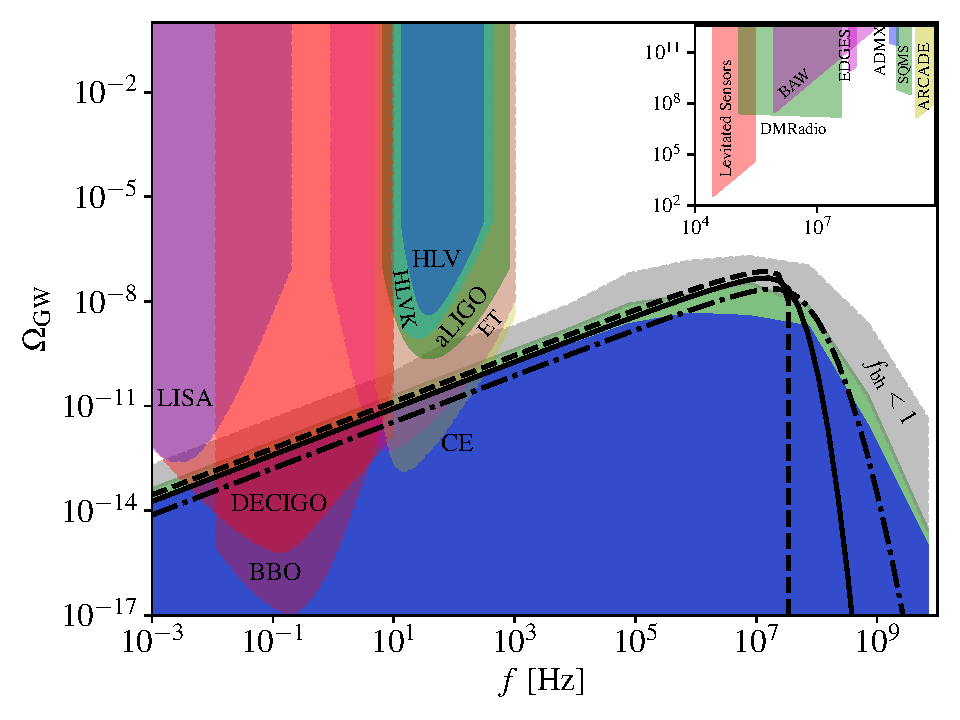
\includegraphics[width=8.5cm]{figs/Merger_GW_posteriors.pdf}}
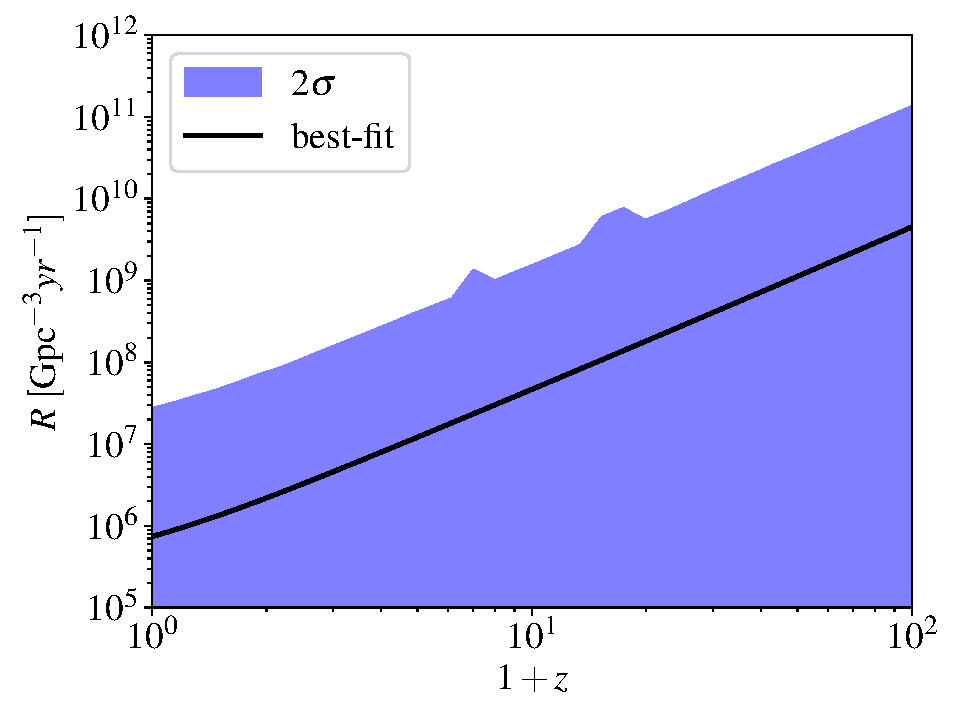
\includegraphics[width=8.5cm]{figs/Merger_rate_posteriors.pdf}}
\caption{
95\% C.L. confidence region for merger $\Omega_\r{GW}$ (left) and merger rate (right) from GW + $\dneff$ + PBH inference,
legend applies to both panels.
The green (blue) regions show the posterior when halo disruption of PBH binary (see \Eq{fduf7ngdygr543}) is ignored (considered).
We also show results when $\fbh < 0.1$ prior has been lifted to $\fbh < 1$ (ignoring the $S_2$ term in \Eq{fduf7ngdygr543}),
however for $\fbh > 0.1$ the robustness of our merger calculation is yet to be verified,
thus we mark these regimes with grey regions.
%the grey regions show the posterior when the $\fbh < 0.1$ prior has been lifted to $\fbh < 1$ (ignoring the $S_2$ term in \Eq{fduf7ngdygr543}),
%in such regimes the robustness of our merger calculation is yet to be tested.
The solid black lines correspond to our best-fit PBH parameters of $\fbh = 10^{-1},\ m_\r{c} = 2.6 \times 10^{-4}m_{\odot},\ \sbh = 0.54$.
In the left panel,
we also show $\Omega_\r{GW}$ computed for $\sbh = 0$ (monochromatic PBHs, dashed) and $\sbh = 1$ (dot-dashed),
with the $\fbh$ and $m_\r{c}$ fixed to 0.1 and $2.6 \times 10^{-4}m_{\odot}$ respectively.
We also show the experimental sensitivities of LISA, DECIGO, BBO, ET, CE, aLIGO, Levitated Sensors, BAW, DMRadio, SQMS and ARCADE.
Sensitivities below kHz frequencies are the power law integrated sensitivities taken from Refs~\cite{Thrane:2013oya, Domenech:2021ztg, Garcia-Bellido:2021jlq},
and sensitivities above kHz are calculated from the strain $h_\r{c}$ sensitivities collected in~\cite{Domcke:2022rgu} via 
$\Omega_\r{GW} = 2 \pi^2 f^2 h_\r{c}^2/(3H_0^2)$~\cite{Thrane:2013oya}.
Existing and proposed experiments are indicated by solid and dashed edges respectively.
The grey dotted line roughly corresponds to the $\Omega_\r{GW}$ upper limit indicated by the PLK $\dneff$ limit of $\dneff < 0.175$
(or $\int \rd \ln f\Omega_{\r{GW}} < 2.1 \times 10^{-6}$~\cite{Cang:2022jyc}).
}
\label{e2f8nb_asadwu}
\end{figure*}

In both panels we also show the result when the $\fbh < 0.1$ prior is lifted to $\fbh < 1$,
which is equivalent to requiring the density of PBH to not exceed that of DM.
It should be note however that the robustness of the $\bar{N}(y)$ expression we used in \Eq{fdvdsx2rsdcvio} is yet to be tested for $\fbh > 0.1$~\cite{Raidal:2018bbj,Hall:2020daa},
thus caution should taken when using our result at such regimes and we indicate these regions with grey colors and dashed edges.
With this caveat in mind,
\Fig{e2f8nb_asadwu} shows that $\fbh < 1$ prior increases the $\GW$ posterior by about a factor of 5 and into the sensitivity reach of 
advanced LIGO (aLIGO)~\cite{Garcia-Bellido:2021jlq} and LISA (Laser Interferometer Space Antenna)~\cite{LISACosmologyWorkingGroup:2022jok},
whereas the posterior for merger rate $R$ is levitated by about a factor of 60.

As structure formation begins,
PBH binaries may collide with DM halos containing PBH clusters~\cite{Vaskonen:2019jpv,Hutsi:2020sol},
which disrupts the binary and thereby suppressing the PBH merger rate at lower redshifts.
This effect can be accounted for by multiplying the differential merger rate in \Eq{dfiiuiu7thxdcyeg63} by an additional suppression term $S_2$~\cite{Hutsi:2020sol},
\be
S_2 \simeq
\r{min}
\left[
1,
1.96
\times
10^{-3}
x^{-0.65}
\exp
\left(
0.03
\ln^2
x
\right)
\right]
\label{fduf7ngdygr543}
\ee
here $x = (t/t_0)^{0.44} \fbh$.
We show results for this scenario in the blue contours of \Fig{e2f8nb_asadwu},
and it can be seen that this lowers $\GW$ posterior by about a factor of 3,
and the corresponding merger rate posterior is reduced to about $R \lesssim 2.6 \times 10^6\ \r{Gpc^{3}yr^{-1}}$.

%
%$\bar{N}(y)$ is the expected number of PBHs within a comoving radius of $r$ around the binary~\cite{Hall:2020daa}.
%Following~\cite{Raidal:2018bbj,Hutsi:2020sol,Hall:2020daa},
%we take 
%$\bar{N}(y) \simeq
%{M \fbh}
%/
%[
%\left<m\right>
%(\fbh + \sigma_\r{M})]
%$,
%which has been shown to agree well with numerical simulation for $\fbh \le 0.1$~\cite{Raidal:2018bbj,Hall:2020daa}.
%Note that however for $\fbh > 0.1$,
%the accuracy of our analytic $\bar{N}(y)$ is yet to be tested,
%and we advise cautions for use of our results in such regimes.

%\section{Conclusions}
\ck{\it Conclusions}
Enhanced curvature perturbation $\ps$ can produce SIGW which serves as a good source candidate of 
the GW signal recently reported by various PTA experiments.
This letter scrutinizes the implication of this scenario at higher frequency band of GW spectrum.
We show that if the PTA GW signal were indeed sourced by SIGW,
the $\ps$ amplitude required will create PBHs in $[2 \times 10^{-5}, 2 \times 10^{-2}]\ m_\odot$ mass range.
Mergers of these PBHs will produce strong GW background across $[10^{-3}, 10^8]$ Hz frequencies,
which falls into the sensitivity reach of various proposed GW projects such as Einstein Telescope (ET),
Cosmic Explorer (CE),
DECIGO and BBO,
thus the high frequency GW experiments can help verify whether the PTA GW signal is sourced by SIGW.

\bigskip

\ck{\it Acknowledgements.}
J.C would like to thank Gabriele Franciolini and Paul Frederik Depta for helpful discussions about data analysis and the calculation of merger GW.

\begin{appendix}
%\onecolumngrid
%
%\section{Mass functions}
%Let's define 
%\be
%\Psi
%\equiv
%\frac{\rd n_\r{bh}}{n_\r{bh} \rd \ln \mbh}
%\label{Nodsfye4yuefg}
%\ee
%and
%\be
%\Phi
%\equiv
%\frac{\rd \rho_{\r{bh}}}{\rho_{\r{bh}} \rd \mbh}
%=
%\frac{\rd n}{\rho_{\r{bh}} \rd \ln \mbh}
%\label{dwuh378yfhj}
%\ee
%
%Note that \Eq{Nodsfye4yuefg} and \Eq{dwuh378yfhj} are conventions used in 2012 and 1812 respectively.
%It can be easily shown that $\Psi$ is related to $\Phi$ by
%%\be
%%\Psi
%%=
%%\frac{\rho_\r{bh}}
%%{n_\r{bh}}
%%\Phi
%%\ee
%
%\be
%\Psi
%=
%P
%\Phi
%,\ 
%P
%=
%\frac{\rho_\r{bh}}
%{n_\r{bh}}
%=
%\left[
%\int \frac{\rd \mbh}{\mbh}
%\Phi
%\right]^{-1}
%\ee
%
%In accordance with 2012,
%let's further define the average of any quantity $F$ by,
%\be
%\left<F\right>
%\equiv
%\int \rd \ln \mbh
%F
%\Psi
%\ee
%
%Expressing this equation in terms of $\Phi$,
%we get
%\be
%\left<F\right>
%=
%P
%\int \rd \ln \mbh
%F
%\Phi
%\ee
%
%In the context of the mass function of this work,
%$\Phi$ is given by,
%\be
%\Phi
%=
%\frac{1}{\sqrt{2 \pi} \sbh \mbh}
%\exp
%\left[
%-
%\frac{\r{ln}^2(\mbh/m_{\r{c}})}
%{2 \sbh^2}
%\right]
%\ee
%and $P$ can be solved analytically
%\be
%P
%=
%\left<
%m\right>
%=
%m_\r{c}
%\r{e}^{-\sbh^2/2}
%\ee
%
%\section{From merger rate to $\Omega_{\r{GW}}$}
%In cosmological convention,
%the $\Omega$ parameter of any energy component $i$ is defined as
%\be
%\Omega_i
%\equiv
%\rho_i/\rho_\r{cr}
%\ee
%However in popular merger GW literatures $\Omega_{\r{GW}}$ in fact refers to $\rd \Omega_{\r{GW}}/\rd \ln f$.
%To avoid confusion we will here use the cosmological convention,
%and for simplicity we will restrict our discussion below to monochromatic PBHs.
%
%%\subsection{Application to monochromatic PBHs}
%\subsection{Integrated $\Omega_{\r{GW}}$}
%The $\Omega_{\r{GW}}$ parameter for GW is defined as,
%\be
%\Omega_\r{GW}
%\equiv
%\rho_\r{GW}
%/
%\rho_\r{cr}
%\ee
%Now let's see how the $\rho_\r{GW}$ term is computed.
%\be
%\begin{aligned}
%\rho_\r{GW}
%&=
%\int_0^{t_0}
%\rd t_r
%R
%E
%\\
%&=
%\int_0^{\infty}
%\frac{\rd z}{(1+z)H}
%RE
%\end{aligned}
%\label{fdf8ey8ew}
%\ee
%here in deriving the second line we have used 
%\be
%\frac{\rd t_r}
%{\rd z}= \frac{-1}{(1+z)H}
%\ee
%$t_0 = 13.8$ Gyr is the current age of the universe,
%$E$ is the \ckk{\bf observed} GW energy released per merger event,
%related to the source frame value $E_s$ by $E = E_s/(1+z)$.
%$R\equiv \rd N/\rd V \rd t$ is the merger rate per unit comoving volume,
%thus $RE$ is the energy release per unit time and volume.
%%Note that $E$ is measured in the observed frame,
%%related to the source frame value $E_s$ by $E = E_s/(1+z)$
%
%\subsection{$\rd \Omega_{\r{GW}}/\rd \ln f$}
%For the sake of clarity,
%we will use subscripts $\ck{r}$ and $\ck{s}$ to denote \ck{redshifted} and \ck{source} quantities,
%quantities without the subscript are the observed quantities.
%The differential $\rd \Omega_{\r{GW}}/\rd \ln f$ now becomes
%\be
%\frac{\rd \Omega_{\r{GW}}}
%{\rd \ln f}
%=
%\frac{f}
%{\rho_\r{cr}}
%\frac{\rd {\rho_\r{GW}}}
%{\rd f}
%\ee
%where ${\rd {\rho_\r{GW}}}/{\rd f}$ is 
%\be
%\frac{\rd {\rho_\r{GW}}}
%{\rd f}
%=
%\int
%\rd t
%R
%\frac{\rd E}
%{\rd f}
%\label{dsfheh8f}
%\ee
%here 
%${\rd E}/{\rd f}$
%is the \ckk{observed} energy $E$ per \ckk{observed} frequency $f$.
%At the source frame,
%the energy spectrum ${\rd E_s}/{\rd f_s}$ is given by \Eq{eqdsfgr89inja},
%\be
%\begin{aligned}
%F(f_s)
%&\equiv
%\frac{\rd E_s}
%{\rd f_s}
%(f_s)
%\\
%&=
%\frac{1}{3}
%(\pi G)^{2/3}
%M^{5/3}
%\eta
%\\
%&
%\times
%\left\{
%\begin{array}{l}
%f_s^{-1/3}
%,
%\ \ \ \ \ \ \ \ \ \ \ \ \ \ \ \ \ \ \ \ \ \ \ \ \ \ \ \  f_s < f_1\\
%\\
%\frac{f_s^{2/3}}
%{f_1}
%,
%\ \ \ \ \ \ \ \ \ \ \ \ \ \ \ \ \ \ \ \ \  \ \ \ \ \ \  f_1 \le f_s < f_2\\
%\\
%\frac{f_s^2}
%{f_1 f_2^{4/3}}
%\frac{f_4^4}
%{\left(
%4(f_\r{r}
%-f_2
%)^2
%+
%f_4^2
%\right)^2
%}
%,  
%\ \ \ \ \  f_2 \le f_s < f_3\\
%\end{array}
%\right.
%\end{aligned}
%\label{eqdsffdrggr89inja}
%\ee
%To get the $\rd E$ in \Eq{dsfheh8f},
%note that due to cosmological redshifting,
%frequency $f$ should have value $f_r = (1+z)f$ at $z$,
%which equals the source frequency for a binary merging at $z$.
%Thus the \ck{source} energy $\rd E_s$ is
%\be
%\rd E_s
%=
%F(f_r)
%\rd f_r
%=
%(1+z)
%F(f_r)
%\rd f
%\ee
%after redshifting,
%current value for $\rd E_s$ should be $\rd E = F(f_r)\rd f$,
%which gives $\rd E/ \rd f = F(f_r)$.
%Inserting this into \Eq{dsfheh8f},
%we get,
%\be
%\frac{\rd {\rho_\r{GW}}}
%{\rd f}
%=
%\int
%\rd t
%R
%F(f_r)
%\label{dsfhdsedfe}
%\ee
%or
%\be
%\frac{\rd \Omega_{\r{GW}}}
%{\rd \ln f}
%=
%\frac{f}
%{\rho_\r{cr}}
%\int
%\frac{\rd z}{(1+z)H}
%R
%F(f_r)
%\label{dsfh763s}
%\ee
%
%

\section{Production of SIGW and PBHs from curvature perturbation}
\begin{figure}[t]
\centering
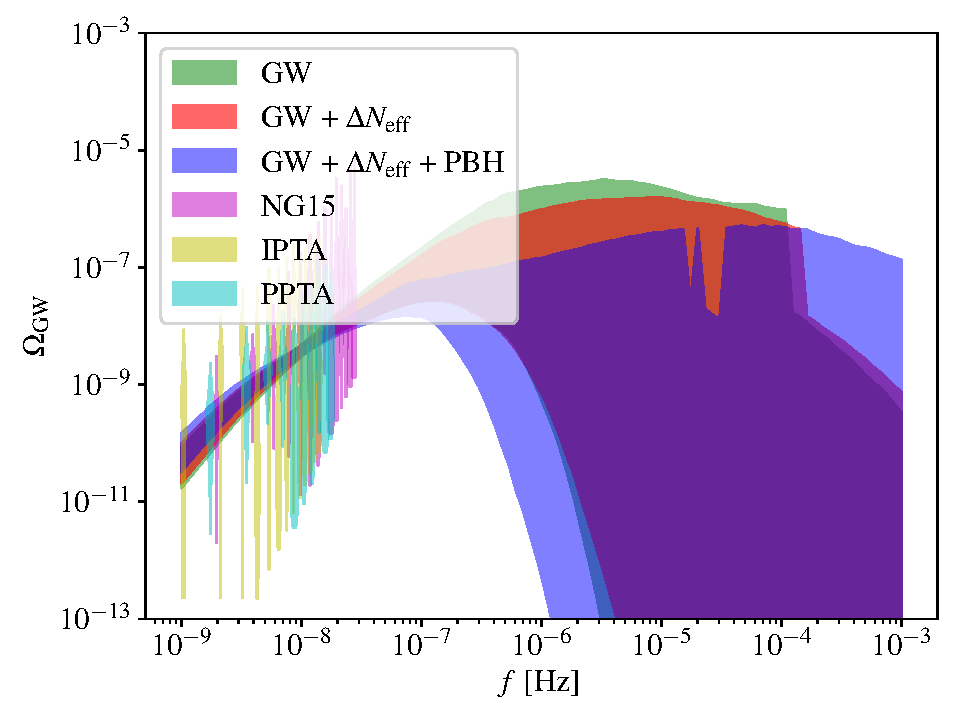
\includegraphics[width=8.5cm]{figs/SIGW_posteriors.pdf}
\caption{
Posterior distribution of SIGW and a comparison with experimental data.
}
\label{e2f8sanb_asadwu}
\end{figure}
%\ck{\it Production of SIGW and PBHs from curvature perturbation}
Upon horizon crossing,
$\ps$ will modify the radiation quadruple moment and generate SIGW at second order,
whose energy density per log frequency interval today is given by~\cite{Cang:2022jyc,Ando:2018qdb,Kohri:2018awv,Inomata:2018epa}

\begin{figure}[t]
\centering
\subfigbottomskip=-200pt
\subfigcapskip=-7pt
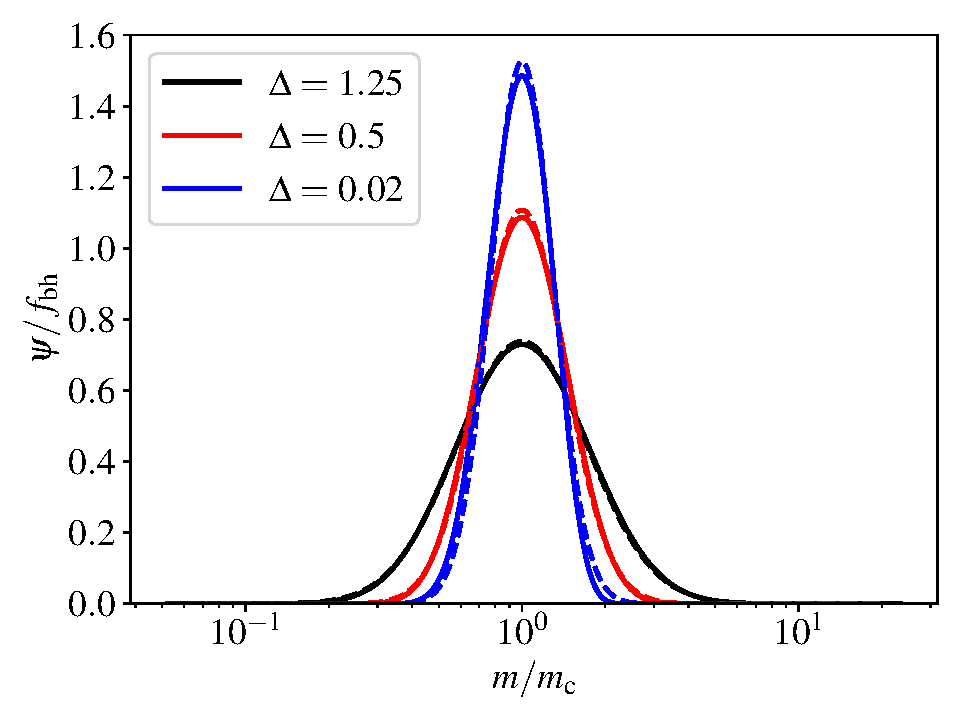
\includegraphics[width=8.5cm]{figs/Phi_compare.pdf}
\caption{
Accuracy of the fit in \Eq{dshiuy65}.
Solid lines show the actual $\psi$ profile computed by \Eq{9876tyuuyt},
dashed lines designate the best-fit log-normal profile using \Eq{dshiuy65}.
In all curves we take $A = 0.1549$ and $k_* = 1.26 \times 10^8 \r{Mpc^{-1}}$.
}
\label{e2f8sasafnb_asadwu}
\end{figure}

\be
\begin{aligned}
\Omega_\r{GW}
&\equiv
\frac{1}{\rho_{\rm cr}}
\frac{{\rm d}\rho_{\rm GW}}{{\rm d}\ln f}
\\
& = 
0.29~
\Omega_{\r{r}}
\left(
\frac{106.75}{g_{\ast}}
\right)^{1/3}
\\
&
\ \ \ \ 
\times
\int^\infty_0 dv \int^{1+v}_{|1-v|} du \left[ \frac{4v^2-(1-u^2+v^2)^2}{4u^2v^2}\right]^2
\\
&\ \ \ \  \times \left(\frac{u^2+v^2-3}{2 u v}\right)^4 F(u,v) \ps(kv)\ps(ku),
\end{aligned}
\ee
\be
\begin{aligned}
F(u,v)
&=
\left( \ln\left| \frac{3-(u+v)^2}{3-(u-v)^2}\right|-\frac{4 u v}{u^2+v^2-3}\right)^2
\\
&
+
\pi ^2 \Theta \left(u+v-\sqrt{3}\right)
,
\end{aligned}
\ee
%$\Omega_{\rm r}=9.1 \times 10^{-5}$ is current radiation density fraction assuming massless neutrinos,
$g_*$ is the total degree of freedom for massless particles when the mode $k$ enters horizon ($k=aH$)~\citep{KolbTurner1990,Wallisch:2018rzj},
$\Theta$ is the Heaviside step function,
and the frequency $f$ is related to the wavenumber $k$ via~\cite{Chen:2021nio},
\be
f = 1.546 \times 10^{-15}\left(\frac{k}{\r{Mpc^{-1}}}\right) \r{Hz}
\ee

%\begin{figure}[tp] 
%\centering
%\subfigbottomskip=-200pt
%\subfigcapskip=-7pt
%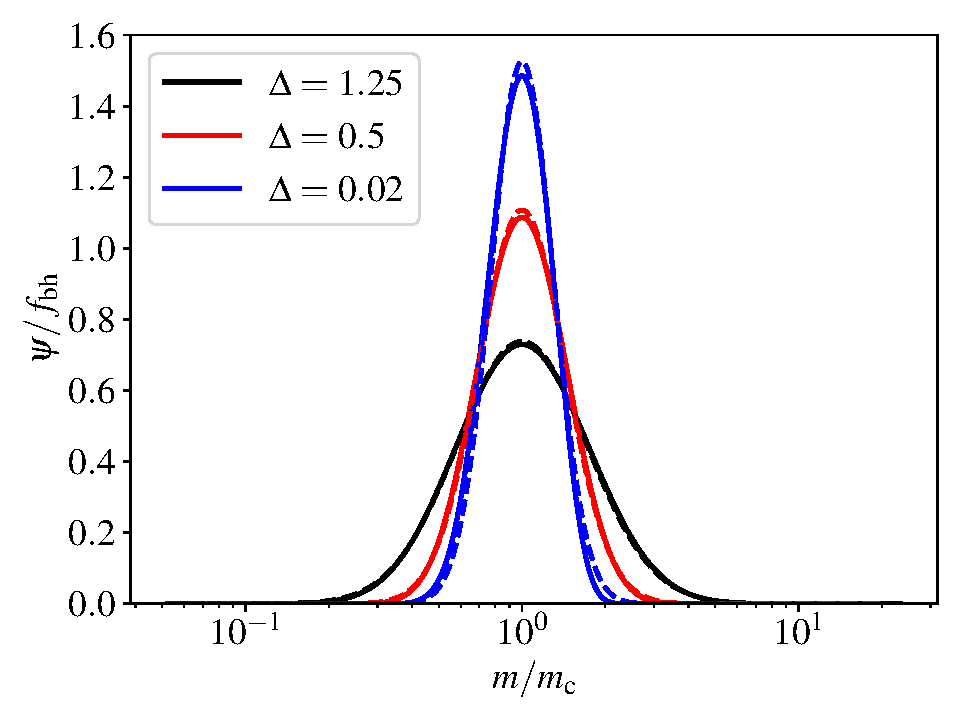
\includegraphics[width=9cm]{figs/Phi_compare.pdf}
%\caption{
%$\Psi$ given by Eq.(\ref{9876tt4erg}) (black) and that calculated using Eq.(\ref{eq98GWenergy01}) (red).
%$\mathcal{P}_S$ is strictly monochromatic in the black line,
%whereas in the red line we have set $\sigma=0.02$ to approximate a sharp semi-monochromatic $\mathcal{P}_S$.
%}
%\label{987ytghyt657fv}
%\end{figure}

In addition to emitting SIGW,
sufficiently large $\ps$ will also generate overdense regions that can gravitationally collapse into PBHs with mass~\cite{Cang:2022jyc,Carr:2009jm,Nakama:2016gzw,Ozsoy:2018flq,Chen:2021nio},
\be
\mbh
=
2.43 \times 10^{-4}
\left(
\frac{\gamma}{0.2}
\right)
\left(
\frac{g_{\ast}}{106.75}
\right)^{-1/6}
\left(
\frac{k}{10^8\rm Mpc^{-1}}
\right)^{-2}
\ms,
\label{k2m_relation}
\ee
here $\gamma$ is the collapse efficiency,
for which we adopt a typical value of $\gamma = 0.2$ following
~\cite{
Carr:2009jm,
Ozsoy:2018flq,
Chen:2021nio}.
The corresponding distribution of PBH abundance is given by~\cite{Carr:2020xqk, Young:2014ana,Ozsoy:2018flq,1975ApJ...201....1C},
\be
\begin{aligned}
\psi
&\equiv
\frac{\r{d}\fbh}{{\rm d} \ln \mbh}
\\
&=
0.28
\left(
\frac{\beta}
{10^{-8}}
\right)
\left(
\frac{\gamma}{0.2}
\right)^{3/2}
\left(
\frac{g_{\ast}}{106.75}
\right)^{-1/4}
\left(
\frac{\mbh}{\ms}
\right)^{-1/2}
,
\label{9876tyuuyt}
\end{aligned}
\ee
where
% $\fbh \equiv \rho_\r{bh}/\rho_\r{dm}$ is the fraction of DM made of PBHs,
%and
\be
\beta (\mbh)
\simeq
\sqrt{
\frac{2 \bar{\sigma}^2}
{\pi \delta_{\rm c}^2}
}
\r{exp}
\left(
-\frac{\delta_{\rm c}^2}{2 \bar{\sigma}^2}
\right),
\label{7865rt54321qw}
\ee
\be
\bar{\sigma}^2
(\mbh)
=
\frac{16}{81}
\int
\r{d}
\ln
k'\,
\left(
\frac{k'}{k}
\right)^4
\ps
(k')
W^2\left(\frac{k'}{k} \right),
\label{8765rfgrtf}
\ee
here $\delta_\r{c}$ is the threshold for gravitational collapse,
for which we adopt 0.45 following~\cite{Cang:2022jyc,Musco:2012au,Harada:2013epa,Carr:2020xqk}.
$W(x)$ is a window function, 
which we use $\exp(-x^2/2)$~\citep{Cang:2022jyc,Ozsoy:2018flq,Chen:2021nio}.

In \Fig{e2f8sanb_asadwu} we show the comparison of SIGW posterior and the PTA data,
\Fig{e2f8sasafnb_asadwu} illustrates the $\psi$ fitting accuracy of \Eq{dshiuy65}.






























\end{appendix}
\bibliography{refs.bib}

\end{document}
